\documentclass[11pt]{article}

\usepackage[letterpaper,margin=1in]{geometry}
\usepackage[T1]{fontenc}
\usepackage[utf8]{inputenc}
\usepackage{lmodern}
\usepackage{microtype}
\usepackage{setspace}
\usepackage{amsmath,amssymb,bm}
\usepackage{booktabs,longtable,tabularx,threeparttable}
\usepackage{graphicx}
\usepackage{pdflscape}
\usepackage{siunitx}
\usepackage{xcolor}
\usepackage{listings}
\usepackage{enumitem}
\usepackage{caption}
\usepackage{url}
\usepackage{natbib}
\usepackage[colorlinks=true,allcolors=blue!55!black]{hyperref}
\usepackage[nameinlink,noabbrev]{cleveref}
\usepackage{fancyhdr}
\hypersetup{
  pdftitle={fereg: Fast, certified high-dimensional fixed-effects regression in Stata},
  pdfauthor={Johannes F. Schmieder},
  pdfkeywords={high-dimensional fixed effects, Stata, least squares, Rust}
}

\newcommand{\fereg}{\texttt{fereg}}
\newcommand{\reghdfe}{\texttt{reghdfe}}
\newcommand{\areg}{\texttt{areg}}
\newcommand{\xtreg}{\texttt{xtreg}}
\newcommand{\stata}{Stata}
\newcommand{\tbu}{\textcolor{red}{\,(\textup{to be updated})}}
\newcommand{\yes}{\textbf{Yes}}
\newcommand{\partialyes}{\textit{Partial}}
\newcommand{\no}{---}
\newcommand{\E}{\mathbb{E}}
\newcommand{\R}{\mathbb{R}}
\newcommand{\trans}{\mathsf{T}}
\newcolumntype{P}[1]{>{\raggedright\arraybackslash}p{#1}}

\captionsetup{font=small,labelfont=bf}
\setlist{nosep}
\onehalfspacing
\setlength{\emergencystretch}{2em}
\pagestyle{fancy}
\fancyhf{}
\fancyhead[L]{\small \fereg}
\fancyhead[R]{\small Working-paper draft}
\fancyfoot[C]{\thepage}

\lstdefinelanguage{Stata}{
  morekeywords={clear,set,generate,replace,bysort,if,in,absorb,vce,
    cluster,predict,assert,display,matrix,list,version,estimates,store,
    fereg,areg,xtreg,reghdfe,quietly,noisily,capture},
  sensitive=true,
  morecomment=[l]{*},
  morecomment=[l]{//},
  morestring=[b]"
}
\lstset{
  language=Stata,
  basicstyle=\ttfamily\small,
  keywordstyle=\color{blue!55!black},
  commentstyle=\color{green!35!black},
  stringstyle=\color{purple!60!black},
  columns=fullflexible,
  keepspaces=true,
  showstringspaces=false,
  breaklines=true,
  frame=single,
  rulecolor=\color{black!25},
  xleftmargin=0.7em,
  xrightmargin=0.7em
}

\title{\texttt{fereg}: Fast, certified high-dimensional fixed-effects
regression in Stata}
\author{Johannes F. Schmieder\thanks{Department of Economics, Boston
University. Email: \href{mailto:johannes@bu.edu}{johannes@bu.edu}.
The public release URL and archival citation are
\href{https://github.com/johannes-schmieder/fereg}
{github.com/johannes-schmieder/fereg}\tbu.}}
\date{August 30, 2026\\[0.5em]\small Working-paper draft}

\begin{document}
\maketitle

\begin{abstract}
\noindent
\fereg\ estimates ordinary and weighted least-squares models with one or
more high-dimensional fixed effects in Stata.  It accepts numeric and
fixed-width string effects, interacted effects, heterogeneous slopes, factor
variables, time-series operators, analytic, frequency, and probability
weights, and one- or multiway clustered covariance estimators.  A thin Stata
control layer delegates data preparation, absorption, finite regression, and
inference to a native Rust plugin, then posts results only after independent
numerical checks pass.  The command provides fast and bounded low-memory
execution, native threading, iterative singleton removal, normalized saved
fixed effects, prediction, and detailed solver and resource diagnostics.
Qualified benchmark receipts compare \fereg\ with a pinned \reghdfe\ 6.14.1
installation and, in a registered low-mobility worker--firm exercise, with
Stata 19's \areg.  In five earlier one- and two-effect
million-observation OLS cells, the geometric-mean
\fereg/\reghdfe\ runtime ratios are 0.304 for fitting and 0.342 when fixed
effects are saved.  Across eight robust and one-way-clustered cells with one
or ten million observations, the ratio is 0.258.  In the registered
worker--firm exercise at eight million observations and four processors,
median elapsed time is 15.9 seconds for \fereg, 263.6 for \reghdfe, and 217.6
for \areg; peak RSS is 3.10, 3.75, and 5.40 GiB, respectively.  These are conditional
engineering results from matched, preflighted SCC shards, not claims of
uniform dominance.  The article describes the estimator, syntax,
postestimation, numerical certificates, feature coverage relative to
\reghdfe\ and Stata's built-in HDFE estimators, and the evidence needed to
interpret the timings.
\end{abstract}

\noindent\textbf{Keywords:} high-dimensional fixed effects; least squares;
multiway clustering; alternating projections; LSMR; Stata; Rust

\noindent\textbf{JEL codes:} C13; C21; C23; C87

\clearpage

\section{Introduction}
\label{sec:introduction}

High-dimensional fixed effects are routine in empirical economics.  A wage
regression may include worker and employer effects
\citep{abowd1999high}; a trade or spatial design may require several
interacted effects; and heterogeneous trends may add a continuous slope for
every unit.  These models are simple to write but expensive to estimate by
forming an explicit dummy-variable matrix.  The difficulty is not the number
of finite coefficients of interest.  It is the size and structure of the
nuisance space that must be removed before those coefficients can be
estimated.

Stata users have several mature ways to approach this problem.  The
\areg\ command has long absorbed a single categorical effect.  Stata 19
extended \areg, \xtreg, and \texttt{ivregress 2sls} to absorb multiple
high-dimensional effects, using Halperin or Cimmino projection methods
\citep{stata2025hdfe,stata2025areg,stata2025xtreg}.  The community-contributed
\reghdfe\ command offers a particularly broad interface: multiple and
interacted effects, heterogeneous slopes, multiway clustering, individual
effects with group-level outcomes, saved effects, and extensive solver
controls \citep{correia2016feasible,correia2026reghdfe}.  Work in Stata and
other statistical systems has made alternating projections a practical
default for this class of models
\citep{guimaraes2010simple,gaure2013ols,somaini2016algorithm}.

\fereg\ is a new Stata command for the linear-model part of this problem.  Its
design has three aims.  First, the hot path should operate in a compiled,
memory-conscious data plane rather than construct large intermediate objects
in ado or Mata.  Second, speed should not be purchased by weakening the
estimation contract: the final sample, coefficient rank, absorbed degrees of
freedom, covariance correction, and saved outputs must remain explicit.
Third, an iterative solver should not be trusted merely because its update
became small.  A successful \fereg\ call must pass fresh projection,
normal-equation, inverse, covariance, and fit checks before Stata's
\texttt{e()} results are changed.

The resulting architecture is deliberately asymmetric.  Stata remains the
control plane: it parses standard syntax, expands the candidate sample, owns
the user-visible transaction, and posts a conventional e-class result.  A
self-contained Rust plugin is the data and computation plane.  One guarded
native call compacts the sample, encodes effects and clusters, removes
singletons, residualizes the outcome and regressors, estimates the finite
coefficients, constructs the requested covariance matrix, recovers optional
fixed effects, validates the complete result, and returns it to Stata.  The
plugin's worker threads never call Stata's plugin interface.

This article contributes a user and technical account of that implementation.
It is not a new estimator of the population parameter.  The estimand follows
the familiar Frisch--Waugh--Lovell decomposition
\citep{frisch1933partial,lovell1963seasonal}; the contribution is a Stata
implementation that combines several certified numerical routes with a
transactional interface, low-memory planning, and reproducible evidence.
The article also draws a careful line between functionality and performance.
Feature coverage is compared with \reghdfe\ 6.14.1, the Stata 19 release
behavior of \areg\ and fixed-effects \xtreg, and the additional functionality
documented in the rolling StataNow channel.  Performance tables compare
\fereg\ with \reghdfe; a new registered scaling exercise compares \fereg,
\reghdfe, and \areg\ on the same worker--firm design.

Two limitations should be clear at the outset.  \fereg\ 0.5 is a linear
estimator.  It does not implement IV/GMM, PPML, other generalized linear
models, HAC or Driscoll--Kraay inference, or individual fixed effects in
group-level outcome data.  These are substantive differences from the
larger \reghdfe\ ecosystem and, in some cases, current StataNow.  In addition,
the benchmark results below describe selected synthetic designs on one
documented Linux/Stata environment.  They establish what happened in those
cells; they do not imply that \fereg\ is faster for every dataset, syntax
combination, operating system, or thread count.

The rest of the article proceeds as follows.  \Cref{sec:model} states the
linear model and sample rules.  \Cref{sec:syntax} introduces the command and
worked examples.  \Cref{sec:coverage} compares features.
\Cref{sec:implementation} describes the native architecture and solvers.
\Cref{sec:inference} covers degrees of freedom and covariance estimation.
\Cref{sec:benchmarks} presents the existing validation and performance
evidence.  \Cref{sec:limits} records current limitations and release
information.  Technical and reproducibility details appear in the appendices.

\section{Model and estimation target}
\label{sec:model}

\subsection{Linear model with absorbed effects}

Let the candidate sample be indexed by $i=1,\ldots,n_0$.  After applying
\texttt{if}, \texttt{in}, missing-value, weight, cluster, and singleton rules,
the estimation sample contains $n$ observations.  On this sample, \fereg\
estimates
\begin{equation}
  y = X\beta + D\alpha + \varepsilon,
  \label{eq:model}
\end{equation}
where $X\in\R^{n\times k}$ contains the finite regressors and $D$ is an
implicit design for the absorbed terms.  For $L$ categorical intercept
effects, $D=[D_1,\ldots,D_L]$.  An absorbed term may also contain
group-specific continuous slopes.  If effect $\ell$ has a categorical
identifier $g_{\ell i}$ and slope variables $z_{\ell i1},\ldots,z_{\ell iq}$,
its observation-level contribution is
\begin{equation}
  d_{\ell i} =
  a_{\ell,g_{\ell i}}+
  \sum_{s=1}^{q} z_{\ell is}c_{\ell s,g_{\ell i}},
  \label{eq:slopes}
\end{equation}
with the intercept omitted for a slope-only term.

Let $W=\operatorname{diag}(w_i)$ denote the objective weights, with
$W=I$ for an unweighted regression.  The coefficient of interest solves
\begin{equation}
  \widehat\beta
   = \arg\min_{\beta}\min_{\alpha}
       (y-X\beta-D\alpha)^\trans
       W(y-X\beta-D\alpha).
  \label{eq:wls}
\end{equation}
Writing $M_D$ for the weighted residual-maker associated with the identified
column space of $D$, the within-regression form is
\begin{equation}
  \widehat\beta
  = (X^\trans W M_D X)^{-}
    X^\trans W M_D y,
  \label{eq:fwl}
\end{equation}
where the inverse is restricted to the numerically identified finite
regressor subspace.  \fereg\ does not build $D$.  Instead, it applies
weighted projections effect by effect, or solves an equivalent implicit
least-squares or graph system.

The finite regression uses scaled column-pivoted Householder QR.  It records a
canonical status for every requested coefficient: identified, base,
omitted/collinear with other finite regressors, or collinear with the
absorbed space.  The reported constant, when structurally present, is a
normalization coordinate,
\begin{equation}
  \widehat\beta_0 =
  \overline y_w-\overline X_w\widehat\beta,
  \label{eq:constant}
\end{equation}
not an additional direction in the finite or absorbed rank.  A model
containing only slope-only absorbed terms therefore need not report a
structural constant.

\subsection{Sample construction and singleton removal}

Sample semantics matter when different commands are compared.  Stata first
applies the user's \texttt{if} and \texttt{in} restrictions and evaluates
factor-variable and time-series expressions.  The plugin then removes rows
with an unavailable outcome, regressor, fixed-effect source, cluster source,
or invalid weight.  Values outside the candidate sample are not inspected.
Probability weights must be strictly positive and select robust inference
when \texttt{vce()} is omitted.  Frequency weights are positive integers and
act as literal multiplicities.  Analytic weights may be rescaled without
changing the fitted coefficients.  Importance weights are recognized only so
that the command can return a fixed, explicit rejection.

By default, \fereg\ removes singleton fixed-effect observations iteratively.
Dropping a singleton in one effect can create a singleton in another, so the
algorithm maintains a queue and continues until no further observation must
be deleted.  The \texttt{keepsingletons} option disables this step.  The
posted \texttt{e(sample)} and singleton counts refer to the final estimation
sample, not the pre-pruning candidate sample.

\subsection{Identified fitted values and normalized effects}

Individual fixed-effect coefficients need not be identified.  In a connected
worker--firm graph, for example, a constant can be moved from every worker
effect to every firm effect without changing a fitted value.  Disconnected
graphs add one such normalization freedom per connected component.
\fereg\ therefore treats
\[
  \widehat d=D\widehat\alpha,\qquad
  \widehat y=X\widehat\beta+\widehat d,
  \qquad\text{and}\qquad
  \widehat\varepsilon=y-\widehat y
\]
as the stable objects.  Saved effect channels are normalized within connected
components and are useful for interpretation or downstream calculations, but
their level is not independently identified.  The command verifies that
their combined contribution reconstructs $\widehat d$ before publication.

\section{Command syntax and use}
\label{sec:syntax}

\subsection{Syntax}

The estimation syntax is
\begin{lstlisting}
fereg depvar [indepvars] [if] [in] [weight], [options]
\end{lstlisting}
where \texttt{weight} may be an analytic, frequency, or probability weight.
The principal options are
\begin{description}[style=nextline,leftmargin=1.5em]
\item[\texttt{absorb(terms)}]
absorb one or more categorical intercept effects, categorical interactions,
or group-specific continuous slopes.  An effect written
\texttt{newvar=effect} also requests a normalized saved channel.
\item[\texttt{vce(unadjusted|robust)} and
\texttt{vce(cluster clustervars)}]
request IID, HC1 robust, or one- to five-way clustered inference.  A
\texttt{\#} inside one cluster term forms a single interacted cluster.
\item[\texttt{dof(pairwise|firstpair|continuous|none)}]
select the absorbed-rank adjustment.  \texttt{pairwise} is the default.
\item[\texttt{residuals(newvar)}]
save estimation residuals.  Residual storage is also required before
\texttt{predict, d}, \texttt{predict, xbd}, or
\texttt{predict, residuals}.
\item[\texttt{solver(auto|map|cg|it|squarem|lsmr|cmg)}]
choose an absorption method.  The default \texttt{auto} route is normally
preferable because it inspects topology, pilot contraction, and the memory
plan.
\item[\texttt{memory(auto|fast|low)} and \texttt{poolsize(\#)}]
select dense reusable workspaces, bounded scratch-backed processing, or an
automatic preflight.  \texttt{poolsize()} controls the regressor block width
in low-memory mode.
\item[\texttt{threads(\#)}, \texttt{deterministic}, and \texttt{timeit}]
control the native thread request, fix partition and merge order on the same
architecture/thread count, and print route, time, memory, RSS, and thread
diagnostics.
\item[\texttt{tolerance(\#)} and \texttt{iterate(\#)}]
set the user tolerance and iteration ceiling.  Exhaustion or a failed
certificate is an error rather than permission to post an approximate result.
\end{description}

The finite regressor list accepts continuous variables, numeric factor main
effects, all-categorical factor interactions, and time-series operators on
continuous variables.  Categorical-by-continuous and
continuous-by-continuous interactions on the right-hand side are not yet
supported.  This restriction concerns finite regressors; heterogeneous
continuous slopes inside \texttt{absorb()} are supported.

\subsection{Installation checks}

Three nonestimation calls help distinguish installation problems from model
problems:
\begin{lstlisting}
fereg, version
fereg, doctor verbose
fereg, selftest
\end{lstlisting}
\texttt{version} checks the ado/plugin protocol handshake.
\texttt{doctor} identifies the loaded artifact and host, and
\texttt{selftest} runs a native diagnostic calculation.  These calls do not
change the data or post estimation results.

\subsection{A two-way fixed-effects regression}
\label{sec:example-basic}

The basic interface follows Stata conventions.  The following synthetic
worker--firm regression absorbs both effects and clusters by firm:
\begin{lstlisting}
clear
set seed 2026082601
set obs 600
generate long worker = ceil(_n/6)
bysort worker: generate byte period = _n
generate long firm = mod(worker + 7*period, 30) + 1
generate double x = rnormal()
bysort worker: generate double worker_fe = rnormal() if _n == 1
bysort worker: replace worker_fe = worker_fe[1]
bysort firm: generate double firm_fe = .7*rnormal() if _n == 1
bysort firm: replace firm_fe = firm_fe[1]
generate double y = 1 + .8*x + worker_fe + firm_fe + rnormal()

fereg y x, absorb(worker firm) vce(cluster firm)
\end{lstlisting}
The coefficient table is conventional, and \texttt{ereturn list} exposes
sample, fit, rank, absorbed degrees of freedom, cluster counts, solver route,
certificate, and resource information.  \texttt{test} operates on the posted
\texttt{e(b)} and \texttt{e(V)}; \texttt{estat summarize} uses
\texttt{e(sample)}.

\subsection{Factors, multiway clusters, and saved effects}

Effects can be named inside \texttt{absorb()}.  Here the two requested
channels, combined absorbed contribution, finite prediction, and residual all
become variables:
\begin{lstlisting}
fereg y x i.region [aw=aw],                         ///
    absorb(fe_worker=worker fe_firm=firm year)      ///
    vce(cluster state#year worker) residuals(ehat)

predict double xb, xb
predict double d, d
predict double xbd, xbd
assert reldif(y, xbd + ehat) < 1e-8 if e(sample)
\end{lstlisting}
In \texttt{vce(cluster state\#year worker)}, \texttt{state\#year} is one
interaction cluster and \texttt{worker} is a second cluster dimension.  It is
different from clustering separately by state and year.  Saved fixed effects
are normalized; \texttt{d}, \texttt{xbd}, and residuals are the more stable
quantities when the effect graph is disconnected or otherwise nonunique.

\subsection{Interacted effects and heterogeneous slopes}

The following syntax absorbs worker intercepts, firm--year cell effects, and
a firm-specific trend:
\begin{lstlisting}
fereg y x, absorb(worker firm#year firm#c.trend) vce(robust)
\end{lstlisting}
The form \texttt{firm\#c.trend} is slope-only.  The shorthand
\texttt{firm\#\#c.trend} instead requests a firm intercept and a firm-specific
trend.  Multiple slopes can be grouped:
\begin{lstlisting}
fereg y x, absorb(worker##c.(trend tenure) firm)
\end{lstlisting}
In the present syntax, categorical \texttt{\#\#} expansion inside
\texttt{absorb()} is not general-purpose.  Users should write desired
categorical main and interaction effects explicitly; the special
\texttt{\#\#c.} form is reserved for an absorbed categorical intercept plus
continuous slopes.

\subsection{Memory and diagnostic controls}

For a large model, the user can request bounded regressor blocks and print the
effective execution plan:
\begin{lstlisting}
fereg y x1-x30, absorb(worker firm)                 ///
    memory(low) poolsize(5) threads(8) timeit
\end{lstlisting}
\texttt{memory(low)} may use temporary scratch storage rather than retain every
within-transformed column.  Scratch files are part of the guarded transaction
and are removed on success, error, or Break.  \texttt{memory(auto)} preflights
the fast and low plans and chooses one that fits.  \texttt{threads(0)} leaves
the native team size automatic; a positive number is a request recorded
alongside the effective count.  \texttt{deterministic} fixes the reduction
partition and merge order for a given architecture and thread count, at a
possible performance cost.

\section{Feature coverage and command choice}
\label{sec:coverage}

\subsection{Why the comparison is versioned}

A feature comparison needs both command and date.  This article pins the
community comparator to \reghdfe\ 6.14.1 at source commit
\texttt{29b2b203f534413369d675d0c0f674d61291f536}
\citep{correia2026reghdfe}.  For official Stata, it separates the Stata 19
release from the current StataNow documentation accessed on August 30, 2026.
StataNow is a continuously updated channel; its column should therefore be
read as a dated snapshot, not as a claim about every installation.

The most important change in Stata 19 was that \areg\ and fixed-effects
\xtreg\ could absorb multiple high-dimensional categorical variables
\citep{stata2025hdfe}.  In \xtreg, the declared panel identifier remains the
first fixed effect, and additional effects are listed in
\texttt{absorb()}.  The commands offer Halperin and Cimmino methods and
pairwise absorbed-degree-of-freedom calculations.  Current StataNow manuals
add richer absorbed interactions and heterogeneous slopes.  They also expand
VCE support: \areg\ includes multiway clustering and HAC options, while
fixed-effects \xtreg\ includes multiway clustering and Driscoll--Kraay
inference; HC2/HC3 variants are available with documented restrictions
\citep{stata2025areg,stata2025xtreg,statanow2026vce}.

\Cref{tab:feature-coverage} gives the detailed comparison.  The label
\emph{Partial} means that the general feature exists but its syntax,
estimator scope, maximum dimensions, or postestimation contract differs
materially.  It is not a quality ranking.  For example, \xtreg\ provides
panel-specific quantities such as $\widehat\sigma_u$, $\widehat\sigma_e$,
$\widehat\rho$, and the fixed-effect test; these are not goals of \fereg.
Conversely, \fereg\ exposes multi-channel saved effects and native memory
diagnostics that the official commands do not.

\subsection{Practical command choice}

For OLS or weighted least squares with several fixed effects, the choice
depends on the requested surface.

\begin{itemize}
\item Use \fereg\ when its supported OLS/WLS surface covers the model and
native threading, low-memory execution, saved channels, or fail-closed
numerical diagnostics are valuable.
\item Use \reghdfe\ when the established ecosystem, group-level outcomes with
individual effects, Driscoll--Kraay inference, or broader compatibility is
needed.  For IV/GMM and Poisson models, the related \texttt{ivreghdfe} and
\texttt{ppmlhdfe} commands cover estimators that \fereg\ 0.5 does not
\citep{correia2020ppmlhdfe}.
\item Use \areg\ when its cross-sectional absorbed-regression interface and
official Stata support are preferable.  In current StataNow, this includes
HAC and other expanded VCE choices subject to the manual's restrictions.
\item Use fixed-effects \xtreg\ when panel declaration, panel variance
components, the unit-effect test, and panel-specific prediction or covariance
estimators are part of the desired result.  Its \texttt{absorb()} option adds
HDFE dimensions to the panel effect rather than turning \xtreg\ into a generic
cross-sectional command.
\end{itemize}

These choices are not mutually exclusive in a validation workflow.  Small
models can be checked against explicit dummy variables, while large
applications can compare samples, finite coefficients, fitted values, and
covariances across applicable commands.  Separate saved fixed-effect
normalizations should not be compared mechanically; their combined fitted
contribution is the identified comparison target.

\section{Implementation}
\label{sec:implementation}

\subsection{Control plane, data plane, and transaction}

\fereg\ follows a narrow control/data-plane boundary.  The ado layer parses
the public syntax, asks Stata to evaluate candidate-sample and expression
semantics, allocates names for requested outputs, and enters a guarded
transaction.  One substantive plugin call then performs the estimation.  The
native result is a complete receipt containing coefficient and covariance
matrices, status vectors, sample indicators, fit and degrees-of-freedom
statistics, fixed-effect and cluster metadata, requested outputs, solver
diagnostics, certificates, and resource measurements.

The order matters.  An error while encoding a string effect, an interrupt
during absorption, a rank failure, an invalid covariance correction, or an
allocation failure must not leave a mixture of old and new results.  Rust
validates dimensions and finite values before exposing the receipt.  The ado
layer posts public variables and \texttt{e()} results only after the receipt
is marked complete.  If anything fails, it restores the pre-call estimation
state and removes temporary variables or scratch files.  Rust panics are
caught at the C boundary rather than unwinding through Stata.

Stata's plugin interface is used only from the calling thread.  After the data
are compacted into Rust-owned storage, native worker threads may perform
projections, cross-products, score reductions, and output construction.  This
restriction avoids calling an interface with uncertain thread-safety from
background workers and makes the host/plugin boundary easier to audit.

\subsection{Data preparation without an explicit dummy matrix}

Every categorical source is mapped to compact integer codes over the final
sample.  Numeric and fixed-width string sources share the same downstream
representation.  Each effect stores level-to-observation membership; an
interaction such as \texttt{firm\#year} is encoded as one categorical
channel.  A slope-bearing level stores the small local design needed for its
intercept and slopes.  Rank-deficient local slope blocks use pivoted
elimination: arbitrary parameter directions may be normalized, but the
projected fitted contribution must remain unique.

The preparation stage also deduplicates fixed-effect and cluster topologies,
labels connected components where needed, and rebases factor recipes after
the final sample is known.  This ordering prevents a base category selected
on the candidate sample from silently disagreeing with the category support
that remains after weight, cluster, or singleton exclusions.

\subsection{Absorption routes}
\label{sec:solvers}

The simplest route is exact one-pass weighted demeaning for one categorical
intercept effect.  Multiple-effect models can use several algorithms:

\begin{description}[style=nextline,leftmargin=1.5em]
\item[Symmetric MAP.]
A complete symmetric Kaczmarz sweep applies the effect projections forward
and backward.  Unaccelerated \texttt{solver(map)} repeats this transform.
\item[Conjugate-gradient acceleration.]
\texttt{solver(cg)} applies conjugate gradients to the positive-semidefinite
complement of the symmetric residual sweep, using a weighted
Fletcher--Reeves recurrence \citep{hestenes1952methods}.  Outcome and
regressor right-hand sides share projection work but maintain separate
recurrences.
\item[Irons--Tuck and SQUAREM.]
\texttt{solver(it)} and \texttt{solver(squarem)} accelerate the fixed-point
map using extrapolation schemes associated with \citet{irons1969version} and
\citet{varadhan2008squarem}.
\item[LSMR.]
\texttt{solver(lsmr)} solves the implicit sparse least-squares problem using
the LSMR recurrence \citep{fong2011lsmr}.  The implementation supports
off, diagonal, and additive Schwarz preconditioners.
\item[CMG-preconditioned graph solve.]
For a two-core-effect categorical graph, \texttt{solver(cmg)} constructs a
graph hierarchy and uses it as a preconditioner for PCG.  The explicit route
allows at most 64 non-base nuisance-effect columns and no absorbed slopes.
Setup or solve failure is visible and falls back to certified CG.
\end{description}

The default \texttt{solver(auto)} is topology- and evidence-based rather than
a fixed alias.  One effect is demeaned directly.  A conservative
worker--firm-like categorical topology can select CMG before a projection
pilot when there are no nuisance Schur columns, at least eight observations
per level of the higher-cardinality core effect, and at least a 10:1 ratio of
core level counts.  Other multi-effect models receive at most four symmetric
MAP pilot sweeps.  A certified pilot ends the solve.  Otherwise, adequate
pilot contraction can select Schwarz-preconditioned LSMR if its complete
workspace fits; remaining cases use CG.  Auto-selected LSMR receives at most
one visible fallback to CG from the saved pilot state.

These routing thresholds are engineering policy, not econometric assumptions.
They can affect runtime and floating-point trajectories, but not the sample,
objective, covariance request, or publication criteria.  The requested and
used routes, pilot information, iteration counts, fallback status, and final
certificate norms are retained in \texttt{e(fereg\_solver)}.

\subsection{Fresh numerical certificates}
\label{sec:certificates}

An iterative recurrence is useful for deciding when to check a candidate; it
is not the final accuracy criterion.  For every effect-level local design
$B$, \fereg\ takes the returned residual $r$, forms the projection of
$W^{1/2}r$ onto $\operatorname{col}(W^{1/2}B)$ using scaled,
reorthogonalized, rank-aware QR, and evaluates its size relative to the
outcome and residual scale.  Normalizing columns before this calculation
makes the check insensitive to units in a slope channel.  A successful
within transformation must pass this fresh, basis-invariant FE-span
certificate.

The finite regression is checked separately.  The implementation recomputes
normal-equation residuals on the identified coefficient subspace, verifies
the QR-based inverse/bread, reconstructs the original-space residual, and
checks fit identities.  Robust and clustered covariance paths add symmetry,
finite-value, correction, and subset checks.  Saved fixed effects must
reconstruct the absorbed target and pass the same FE moment condition.
Iteration exhaustion, nonfinite curvature, a failed fresh projection, or
nonpositive residual degrees of freedom ends the command with an error.

This approach is intentionally redundant.  The algorithm that produced a
candidate and the calculation that certifies it do not share the same stopping
recurrence.  A bug in a recurrence or an apparently stable but inaccurate
fixed point is therefore less likely to become a posted estimate.

\subsection{Fast and low-memory execution}

\texttt{memory(fast)} retains within-transformed columns and reusable native
workspaces.  It is the natural choice when memory is ample and a moderate or
large finite regressor list will be processed repeatedly.  In
\texttt{memory(low)}, regressors and scores are handled in blocks, with
bounded scratch-backed storage when required.  The scientific stages and
publication gates are the same in both modes.

Before large allocation, the command checks dimensions and estimates
route-specific storage.  \texttt{memory(auto)} chooses a feasible plan rather
than starting a fast allocation and silently degrading after partial work.
The diagnostic matrix \texttt{e(fereg\_runtime)} records the plan, native
allocation, scratch usage, timing stages, RSS observations, and requested and
effective thread counts.  These quantities are useful for reproducible
performance reports, but RSS remains an operating-system measurement rather
than an exact allocator identity.

\section{Degrees of freedom and covariance estimation}
\label{sec:inference}

\subsection{Absorbed rank}

Residual degrees of freedom combine the effective sample size, the rank of
the finite regression, and the rank contributed by the absorbed design.  With
one categorical intercept effect, the absorbed rank follows directly from
the number of supported levels and the intercept convention.  With two
effects, connected components of the bipartite graph identify exact
redundancies.  With more effects, exact global rank can be substantially more
expensive than estimation, so \fereg\ exposes policies that parallel common
HDFE practice.

\texttt{dof(pairwise)}, the default, uses pairwise connected-component
calculations to account for redundancies across effect dimensions.
\texttt{dof(firstpair)} performs the graph calculation for the first pair and
uses bounded adjustments thereafter.  \texttt{dof(continuous)} additionally
accounts for local rank in slope-bearing terms.  \texttt{dof(none)} applies
no redundancy recovery beyond the basic count.  The selected policy and
component information are posted.  Successful inference requires
$df_r>0$.

If an absorbed effect is nested in a cluster dimension, the finite-sample
cluster correction avoids charging the same variation twice.  This nesting
logic is evaluated on the final sample and is part of the covariance
certificate, not an after-the-fact label.

\subsection{IID and HC1 covariance}

Let $\widetilde X=M_DX$ contain the identified within regressors and define
\[
  B=(\widetilde X^\trans W\widetilde X)^{-}.
\]
For IID inference, \fereg\ reports
\begin{equation}
  \widehat V_{\mathrm{IID}}
  = \frac{\widehat\varepsilon^\trans W\widehat\varepsilon}{df_r}B.
  \label{eq:iid}
\end{equation}
For robust inference, observation-level score vectors are accumulated using
the command's weight-specific score convention.  If $s_i$ denotes the
identified-coordinate score, the HC1 form is
\begin{equation}
  \widehat V_{\mathrm{HC1}}
  = c_{\mathrm{HC1}} B
      \left(\sum_{i=1}^{n}s_i s_i^\trans\right)B,
  \label{eq:hc1}
\end{equation}
where the finite-sample multiplier is determined by effective sample and
model degrees of freedom.  The implementation centralizes this correction so
that unweighted, analytic, frequency, and probability-weight paths cannot
quietly apply inconsistent counts.

\subsection{One- and multiway clustering}

For a cluster dimension $g$, define the cluster score
$S_g=\sum_{i\in g}s_i$.  The one-way meat is
\[
  M_g=\sum_g S_gS_g^\trans.
\]
For $J$ cluster dimensions, \fereg\ uses inclusion--exclusion
\citep{cameron2011robust}.  If $A$ is a nonempty subset of the dimensions and
$M_A$ is the meat obtained by clustering on their joint cells, then
\begin{equation}
  M_{\mathrm{multi}}
  = \sum_{\varnothing\ne A\subseteq\{1,\ldots,J\}}
      (-1)^{|A|+1}c_A M_A,
  \qquad
  \widehat V_{\mathrm{multi}}=BM_{\mathrm{multi}}B.
  \label{eq:multiway}
\end{equation}
The public interface accepts up to five declared dimensions.  Interacted
syntax inside one dimension does not increase this count.  Cluster counts,
subset structure, corrections, nesting decisions, and any numerical
positive-semidefinite repair are recorded in \texttt{e()} results.

\fereg\ 0.5 does not implement HC2/HC3, HAC, or Driscoll--Kraay covariance
estimators.  Users requiring them should choose a command that implements the
desired estimator and check the applicable restrictions.  In particular,
current StataNow documents limitations on HC2/HC3 and HAC when more than one
effect is absorbed \citep{stata2025areg,stata2025xtreg,statanow2026vce}.

\section{Validation and benchmark evidence}
\label{sec:benchmarks}

\subsection{What counts as benchmark evidence}

The tables are generated from existing immutable evidence bundles in the
repository.  The two figures use a dedicated registered benchmark executed
for this article.  After that run completed, its receipts were frozen; the
figure generator reads only the captured bundle and cannot invoke Stata or the
scheduler.  Both generators check source and plugin identities, expected cell
and preflight counts, terminal success status, and input-file hashes before
producing LaTeX.  This protects the manuscript from copying an orphaned
timing number without its associated scientific and operational checks.

The comparison command is \reghdfe\ 6.14.1 from the pinned source described in
\Cref{sec:coverage}.  The OLS evidence uses \fereg\ source
\texttt{947f79373306760a635494935cc84c0f5ebfcda8} and Linux plugin SHA-256
\texttt{94017d23d97c1a0890cd9a1a180dad4ce3482b5b29cbe6efdbece5016b3e7099}.
The VCE evidence uses source
\texttt{490e03a3e2458d8bc463c3f60389062e2f8fae42}, source-archive SHA-256
\texttt{4f4e44cc539419ae67043cfca824c92aed7c6b1969c1a37825939e2397d02aab},
and plugin SHA-256
\texttt{9cbe00b6c5a0d5c47af3d5d1fd32166a200d27202d335a602d584a3d5b48a4a2}.
These identities attach the results to the tested artifacts; they should not
be relabeled as evidence for a later release commit.

Each reported cell is a within-shard warm median.  The compared commands use
the same generated dataset and requested model.  A preflight checks the
effective sample and singletons, coefficient and omission structure,
covariance and absorbed degrees of freedom, requested outputs, fit
reconstruction, and registered numerical tolerances.  A timing is retained
only after that preflight passes.  Five OLS shards contributed 180 timing rows
and five passing preflights.  Eight VCE shards contributed 72 timing rows and
eight passing preflights.  The final shards had zero command and scientific
failures and successful scheduler accounting.

The earlier benchmark harness contained another diagnostic arm.\footnote{The harness
also included gtools' \texttt{gregress} 1.11.8.  Because
\texttt{gregress} is explicitly beta and does not expose the full e-class
contract used for these checks, it is not used for feature or headline
performance claims.}  It is omitted from the manuscript tables.  \areg\ is
also omitted from those tables because it was absent from the underlying
qualified evidence bundles; the registered scaling figures below include a
separately qualified Stata 19 \areg\ arm.
An earlier broad development run completed only 100 of 116 intended scopes;
the missing scopes included many of the most expensive cases.  Summarizing
that partial run would invite selection bias, so it is not used here.

\subsection{Scaling in observations and cores}

\begin{figure}[tbp]
\centering
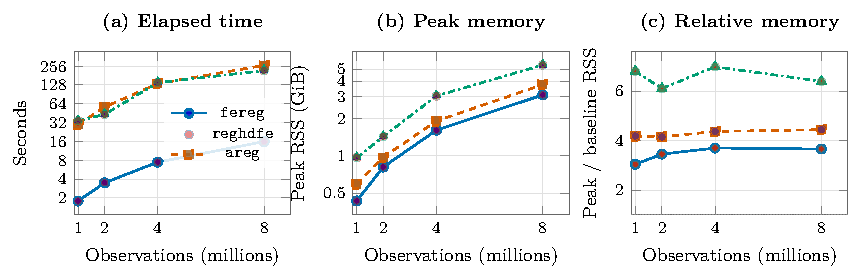
\includegraphics[width=\textwidth]{figures/akm_size_memory.pdf}
\caption{Scaling with the number of observations.  Each line is one complete
command call in a low-mobility two-way worker--firm model with ten finite
controls and default IID inference.  All three commands receive four Stata
processors; \fereg\ also receives four native threads.  Points are medians of
five fresh Stata processes and whiskers span the minimum and maximum.  Panel
(a) reports elapsed command time, panel (b) the peak resident set size (RSS)
sampled externally at 0.01-second intervals, and panel (c) peak RSS divided by
the median RSS after loading the data but before invoking the regression.
Time and peak-memory axes are logarithmic.  Data construction fixes ten
periods per worker, twenty initial workers per firm, and a period-to-period
mobility probability of 0.02.}
\label{fig:akm-size-memory}
\end{figure}

\begin{figure}[tbp]
\centering
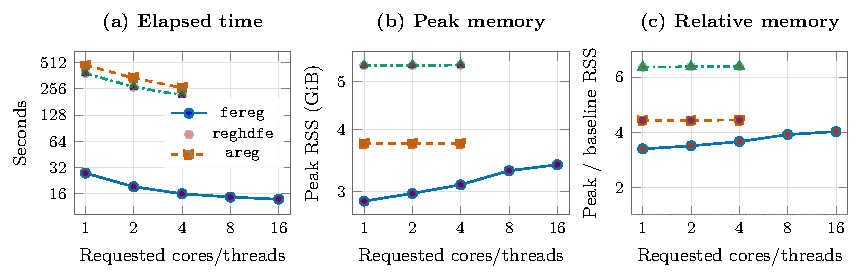
\includegraphics[width=\textwidth]{figures/akm_core_memory.pdf}
\caption{Scaling with requested cores or native threads at eight million
observations.  The data, model, inference, fresh-process repetitions, external
RSS measurement, and panel definitions are the same as in
\Cref{fig:akm-size-memory}.  \fereg\ is measured with 1, 2, 4, 8, and 16
effective native threads.  The \reghdfe\ and \areg\ lines end at four because
four Stata processors were available under the installed license; their
absence at 8 and 16 is a resource constraint, not a failed or selectively
discarded measurement.  The horizontal axis and the time and peak-memory
axes are logarithmic.}
\label{fig:akm-core-memory}
\end{figure}

The figure exercise uses \fereg\ source
\texttt{490e03a3e2458d8bc463c3f60389062e2f8fae42}, plugin SHA-256
\texttt{9cbe00b6c5a0d5c47af3d5d1fd32166a200d27202d335a602d584a3d5b48a4a2},
and the same pinned \reghdfe\ 6.14.1 source.  Its 23 cells contain five
independent command processes each, for 115 measurements in randomized
order.  Eleven untimed parity preflights cover every \fereg\ sample-size and
thread combination and compare the estimation sample, coefficients,
covariance matrix, residual sum of squares, absorbed degrees of freedom, and
residuals with both comparators.  All eleven gates pass before the timing
matrix begins.  Dataset loading and a one-second baseline stabilization are
outside the reported command time.

At the equal four-processor allocation in \Cref{fig:akm-size-memory}, \fereg\
has the lowest median elapsed time and peak RSS at every sample size.  Its
median runtime advantage ranges from 16.2 to 18.0 times relative to
\reghdfe\ and from 12.4 to 19.2 times relative to \areg.  At eight million
observations, the medians are 15.929, 263.629, and 217.594 seconds for
\fereg, \reghdfe, and \areg, respectively.  Peak RSS in that cell is 3.097
GiB for \fereg, compared with 3.752 GiB for \reghdfe\ and 5.398 GiB for
\areg.  Thus \fereg's peak is 17 percent below \reghdfe's and 43 percent
below \areg's in this cell.  Relative to the loaded-process baseline, the
three peaks are 3.659, 4.441, and 6.390.

The core-scaling results in \Cref{fig:akm-core-memory} show both the gain and
the cost of native threading.  Raising \fereg's effective thread count from
one to four reduces the eight-million-observation median from 27.513 to
15.929 seconds.  Moving from four to sixteen threads reduces it further, to
13.784 seconds, for an overall one-to-sixteen speedup of 2.00.  Over the same
range, peak RSS rises from 2.871 to 3.399 GiB and the peak-to-baseline ratio
rises from 3.394 to 4.023.  The extra threads therefore improve time in this
design, but with diminishing returns and a measurable memory cost.  The
figures describe this registered synthetic workload; they do not establish
the same ranking or scaling rate for every fixed-effect graph or machine.

\subsection{OLS fit and saved-effect cells}

\begin{table}[tbp]
\centering
\caption{Existing OLS benchmark evidence: \texttt{fereg} versus \texttt{reghdfe}}
\label{tab:bench-ols}
\small
\begin{threeparttable}
\begin{tabular}{llrrrrr}
\toprule
Design & Mode & $K$ & Threads & \texttt{fereg} & \texttt{reghdfe} & Ratio \\
\midrule
Worker--firm & Fit & 30 & 1 & 5.080 & 25.424 & 0.200 \\
Worker--firm & Fit + save FE & 30 & 1 & 5.939 & 29.473 & 0.202 \\
Worker--firm & Fit & 30 & 16 & 2.129 & 11.958 & 0.178 \\
Worker--firm & Fit + save FE & 30 & 16 & 2.448 & 12.474 & 0.196 \\
One FE & Fit & 10 & 1 & 1.438 & 2.204 & 0.652 \\
One FE & Fit + save FE & 10 & 1 & 1.910 & 2.749 & 0.695 \\
One FE & Fit & 30 & 1 & 3.210 & 8.245 & 0.389 \\
One FE & Fit + save FE & 30 & 1 & 4.026 & 8.697 & 0.463 \\
One FE & Fit & 30 & 16 & 1.424 & 4.967 & 0.287 \\
One FE & Fit + save FE & 30 & 16 & 2.002 & 5.438 & 0.368 \\
\midrule
\multicolumn{4}{l}{Geometric mean, fit cells} & \multicolumn{2}{r}{ } & 0.304 \\
\multicolumn{4}{l}{Geometric mean, fit + save FE cells} & \multicolumn{2}{r}{ } & 0.342 \\
\bottomrule
\end{tabular}
\begin{tablenotes}[flushleft]\footnotesize
\item Notes: Seconds are within-shard warm medians. All designs have $N=1{,}000{,}000$. Worker--firm models have two absorbed effects and 30 finite controls; one-FE models have 10 or 30 controls. Ratio is \texttt{fereg}/\texttt{reghdfe}; values below one favor \texttt{fereg}. Threads are the requested native \texttt{fereg} threads. The 16-thread shards ran Stata/IC with four Stata processors. Source and scientific gates are described in Section~\ref{sec:benchmarks}.
\end{tablenotes}
\end{threeparttable}
\end{table}


\Cref{tab:bench-ols} contains five design/thread cells, each in fit-only and
fit-plus-saved-effects modes.  All have one million observations.  The
two-effect design is a standard synthetic worker--firm graph with 30 finite
controls.  The other design has one absorbed effect and either 10 or 30
controls.  Within these cells, the \fereg/\reghdfe\ ratios range from 0.178 to
0.652 for fitting and from 0.196 to 0.695 when fixed effects are saved.
\fereg\ is faster in all five cells of each mode.  The geometric-mean ratios
are 0.304 and 0.342, respectively.

The saving comparison includes the work required to return requested
normalized effects, not only the within regression.  This distinction is
important because effect recovery can become a second large numerical
problem.  \fereg\ retains a compatible coefficient-space product on several
fast routes and otherwise performs a separately certified recovery; the cost
is therefore route-dependent.

\subsection{Robust and clustered cells}

\begin{table}[tbp]
\centering
\caption{Existing robust and clustered benchmark evidence}
\label{tab:bench-vce}
\small
\begin{threeparttable}
\begin{tabular}{llrrrr}
\toprule
$N$ & VCE & Threads & \texttt{fereg} & \texttt{reghdfe} & Ratio \\
\midrule
1m & HC1 robust & 1 & 10.982 & 46.182 & 0.238 \\
1m & HC1 robust & 16 & 3.000 & 14.086 & 0.213 \\
1m & Cluster (one way) & 1 & 6.875 & 25.006 & 0.275 \\
1m & Cluster (one way) & 16 & 4.437 & 30.308 & 0.146 \\
10m & HC1 robust & 1 & 161.455 & 442.199 & 0.365 \\
10m & HC1 robust & 16 & 87.216 & 369.233 & 0.236 \\
10m & Cluster (one way) & 1 & 131.854 & 350.998 & 0.376 \\
10m & Cluster (one way) & 16 & 60.488 & 205.534 & 0.294 \\
\midrule
\multicolumn{5}{l}{Geometric mean across eight cells} & 0.258 \\
\bottomrule
\end{tabular}
\begin{tablenotes}[flushleft]\footnotesize
\item Notes: Seconds are within-shard warm medians for worker--firm models with 30 finite controls. Ratio is \texttt{fereg}/\texttt{reghdfe}. Every shard ran on a 32-processor SCC node. Stata/IC used one processor in the one-thread cells and four processors in the 16-thread cells; the native \texttt{fereg} request was validated separately. See Section~\ref{sec:benchmarks} for scope and qualification cautions.
\end{tablenotes}
\end{threeparttable}
\end{table}


\Cref{tab:bench-vce} reports worker--firm models with 30 finite controls at one
and ten million observations.  The covariance is HC1 robust or clustered on
one dimension.  The \fereg/\reghdfe\ ratios range from 0.146 to 0.376, with a
geometric mean of 0.258 across eight cells.  \fereg\ is faster in all eight
reported cells.

The thread labels require care.  Every final shard ran on a 32-processor SCC
node under Stata 19/IC.  In the cells labeled 1, both the requested native
\fereg\ count and Stata processor count were one.  In cells labeled 16,
\fereg\ was asked to use 16 native threads and the request was checked, while
Stata/IC reported four Stata processors.  Thus the high-thread results are
useful measurements of the available commands in that licensed environment,
not a controlled claim about equal core counts.  The one-thread cells provide
the cleaner single-core comparison.

\subsection{Interpretation}

The reported ratios are large enough to be practically meaningful in the
selected designs, but neither the tables nor figures are a statistical experiment over the
space of possible datasets.  They use synthetic topologies, fixed regressor
counts, one Stata flavor, Linux x86-64, and particular qualified source
revisions.  Runtime can change with connectivity, effect cardinalities,
slope blocks, condition number, requested outputs, clustering dimensions,
weights, memory pressure, compiler target, and thread scheduling.

The benchmark also compares complete command calls, not a claim that one
specific algorithm is always faster.  \fereg\ may choose direct demeaning,
MAP, LSMR, CG, or CMG, and \reghdfe\ has its own solver and memory controls.
Neither the geometric mean nor the fact that every listed ratio is below one
licenses extrapolation to unsupported model classes or unmeasured platforms.
A user with a consequential application should validate the exact model on
representative data, inspect samples and scientific outputs, and then time
repeated calls.

\section{Limitations, availability, and release status}
\label{sec:limits}

\subsection{Current limits}

The current public surface is intentionally narrower than the most mature
comparators.

\begin{itemize}
\item The estimator is OLS/WLS.  IV/GMM, PPML, other generalized linear
models, and group outcomes with individual fixed effects are unsupported.  A
packaged \texttt{feppml} name is a fail-closed stub, not an experimental
estimator.
\item Inference is IID, HC1 robust, or one- to five-way clustered.  HC2,
HC3, HAC, and Driscoll--Kraay are not implemented.
\item Finite right-hand-side syntax does not yet include
categorical-by-continuous or continuous-by-continuous interactions.  These
must not be confused with supported absorbed heterogeneous slopes.
\item Fixed-width string categorical sources are supported, but
\texttt{strL} sources are not.  Explicit factor base overrides are restricted
when absorption includes interacted or slope-bearing effects.
\item There is no GPU route.  Native threading is local to a command call.
Deterministic execution fixes reductions only for the same architecture and
thread count; it is not a promise of bitwise equality across platforms.
\item Only Stata 18 and newer are supported.  A platform plugin is required,
and an artifact qualified on one operating system or architecture is not
evidence for another.
\end{itemize}

Unsupported public requests fail with an error.  They do not switch silently
to an undocumented ado/Mata estimator or a looser numerical tolerance.

\subsection{Availability and license}

The planned public release is version 0.5.0 at
\url{https://github.com/johannes-schmieder/fereg}\tbu.  It will be distributed
under the GNU General Public License, version 3.0 only (GPL-3.0-only); the
repository's license files and dependency notices will be synchronized before
release\tbu.  The archival release date, DOI, exact release commit, and
platform artifact checksums remain to be frozen\tbu.

The package targets Stata 18 and 19 on Linux x86-64, Windows x86-64, macOS
Apple Silicon, and macOS Intel through a universal binary.  Completed
release-candidate qualification across those targets remains
\tbu.  Benchmark evidence in this article is narrower: it is Linux x86-64
under Stata 19/IC and belongs to the exact artifacts identified in
\Cref{sec:benchmarks}.

\section{Conclusion}
\label{sec:conclusion}

\fereg\ brings a native, threaded data plane to high-dimensional
fixed-effects OLS and weighted least squares in Stata while retaining an
ordinary Stata command and postestimation interface.  Its defining
implementation choices are not only the set of fast absorption routes.  They
also include final-sample encoding, rank-aware finite regression, explicit
degrees-of-freedom policy, transactional posting, low-memory planning, and
fresh numerical certificates that can reject an apparently converged result.

The command already covers many common empirical designs: multiple and
interacted effects, heterogeneous slopes, factor variables, time-series
operators, three public weight types, multiway clustering, iterative singleton
removal, saved normalized effects, and prediction.  It does not yet replace
the broader \reghdfe\ ecosystem or the panel-specific and newer covariance
features in current StataNow.  The feature table is meant to make those
boundaries visible rather than imply a single winner for every application.

Qualified SCC receipts show substantial runtime advantages over \reghdfe\ in
the one- and two-effect OLS, saved-effect, robust, and one-way clustered cells
reported here, while the registered worker--firm figures add an equal-resource
comparison with Stata 19's \areg\ and a separate view of native thread
scaling.  The evidence is deliberately versioned, preflighted, and limited to
its tested environments.  Future release work
should preserve that discipline: new performance claims should follow
scientific parity, attach to exact artifacts, and distinguish complete
qualified matrices from exploratory or incomplete runs.

\section*{Acknowledgments}

The author thanks the developers of Stata's HDFE commands, \reghdfe,
\texttt{ftools}, and the numerical libraries on which this implementation
builds.  Additional acknowledgments will be added before submission\tbu.

\clearpage
\appendix

\section{Technical details}
\label{app:technical}

\subsection{Weighted projection kernel}

For an intercept-only effect with levels $g=1,\ldots,G$, the weighted
projection of a vector $v$ onto the effect space replaces each observation by
its group mean,
\[
  (P_gv)_i =
  \frac{\sum_{j:g_j=g_i}w_jv_j}
       {\sum_{j:g_j=g_i}w_j}.
\]
The residual operator is $I-P_g$.  Multiple nonorthogonal effects require
iterating these operators.  A symmetric sweep applies residual operations in
forward and reverse order, producing a self-adjoint map under the weighted
inner product.  This structure permits the conjugate-gradient acceleration
described in \Cref{sec:solvers}.

For an intercept-plus-slope effect, each level solves a small weighted
least-squares problem.  Let $B_g$ contain the local intercept and slope
columns.  The projected values are
\[
  B_g(B_g^\trans W_gB_g)^{-}B_g^\trans W_gv_g.
\]
The local inverse is rank revealing.  Thus a slope with no within-level
variation does not cause an arbitrary inverse or contaminate the fitted
projection.

\subsection{CG recurrence and independent publication}

Let $M$ be one symmetric residual sweep and $\Pi=I-M$.  The CG route starts
from $r_0=\Pi y$ and $u_0=r_0$.  At iteration $j$ it forms
$v_j=\Pi u_j$ and, for each active right-hand side, computes
\[
  a_j=\frac{\langle r_j,r_j\rangle_W}
            {\langle u_j,v_j\rangle_W},
  \qquad
  y_{j+1}=y_j-a_ju_j,
  \qquad
  r_{j+1}=r_j-a_jv_j.
\]
The next direction uses the Fletcher--Reeves ratio.  A finite nonpositive
curvature caused by lost conjugacy triggers a restart from the true residual;
nonfinite recurrence values are fatal.  Right-hand sides that have already
passed their own condition can be deactivated while others continue.

The ordinary route requires both its energy-based recurrence condition and
the fresh FE-span certificate in \Cref{sec:certificates}.  Coefficient
recovery for saved effects adds an observation-space reconstruction
condition,
\[
  \frac{\max_i|t_i-(D\widehat\alpha)_i|}
       {\max_i|t_i|}
  \leq \min(10^{-10},\text{the stricter tolerance-derived bound}),
\]
with the usual safe convention when the denominator is zero.  Recovery may
continue from an already useful CG state; it does not discard the fit merely
to start an unrelated second solve.

\subsection{Automatic routing details}

The automatic route uses the following hierarchy:
\begin{enumerate}
\item Demean one categorical intercept effect directly and certify it.
\item For eligible two-core-effect categorical graphs, attempt CMG before a
MAP pilot.  Eligibility requires no nuisance Schur columns, at least eight
observations per level of the larger effect, and a 10:1 core
cardinality ratio.
\item Otherwise run at most four symmetric MAP pilot sweeps.  Return if the
fresh certificate passes.
\item If pilot contraction is at least 0.008 and the complete workspace fits,
run direct Schwarz-preconditioned LSMR at internal tolerance
$\max(10^{-14},10^{-2}\tau)$, where $\tau$ is the requested tolerance.
\item Use CG for remaining cases.  An auto-selected LSMR failure may fall back
once to CG within the remaining iteration and memory budget.
\end{enumerate}
All paths end at the same independent publication checks.  The constants above
are frozen routing policy for version 0.5, not user-facing convergence
guarantees.

\subsection{Saved-effect recovery}

Saving effects can dominate runtime if it repeats the absorption problem.
\fereg\ therefore retains coefficient-space products when the selected route
makes them available.  LSMR retains its coefficient vectors.  The CMG route
converts exposed graph potentials and combines them with nuisance-effect
solutions.  CG carries compact effect coefficients through the same
recurrence as its observation-space directions.  Intercept-only MAP
accumulates group coefficients during the original sweeps.

When no retained product is available, including some low-memory paths, the
command runs a bounded reconstruction-aware recovery and then a certified
fallback if needed.  Every result is normalized by connected component,
scattered only for requested channels, reconstructed in observation space,
and checked against the target absorbed contribution.  A convenient saved
normalization never substitutes for the identified fitted-value check.

\subsection{Finite regression, weights, and covariance}

After absorption, scaled column-pivoted Householder QR identifies the finite
regressor rank.  The command keeps the requested coefficient slots so that
Stata factor-variable names and omission status remain interpretable.  It
solves and forms bread only on the identified coordinates, then embeds the
result in the requested coefficient layout.

Weight types differ in more than syntax.  Frequency weights change effective
counts as literal row replication would.  Analytic weights describe
precision and are scale invariant for point estimates.  Probability weights
require robust or clustered inference.  These distinctions feed the
effective sample, residual degrees of freedom, score construction, and
finite-sample corrections; one generic square-root-weight transformation is
not treated as a complete inferential specification.

Multiway clustering builds one score reduction for every nonempty subset of
declared dimensions.  The inclusion--exclusion signs in
\Cref{eq:multiway} are applied after subset counts and corrections are
validated.  At five dimensions there are $2^5-1=31$ subset meats, which makes
bounded score storage and deduplicated topology important.

\subsection{Returned results}

In addition to standard \texttt{e(b)}, \texttt{e(V)}, \texttt{e(sample)},
sample size, rank, fit statistics, and residual degrees of freedom, \fereg\
posts the following structured diagnostics:
\begin{description}[style=nextline,leftmargin=1.5em]
\item[\texttt{e(fereg\_solver)}]
requested and used solver, pilot and iteration counts, fallback, stop reason,
and convergence measures;
\item[\texttt{e(fereg\_runtime)}]
memory plan, native allocation, scratch and RSS diagnostics, timing stages,
and requested/effective threads;
\item[\texttt{e(fereg\_certificate)}]
independent projection, normal-equation, inverse, reconstruction, and related
numerical checks;
\item[\texttt{e(fereg\_dof)}, \texttt{e(fereg\_fe)}, and
\texttt{e(fereg\_cluster)}]
absorbed-rank policy, effect topology, nesting, cluster dimensions, and subset
counts; and
\item[\texttt{e(fereg\_status)} and \texttt{e(fereg\_subset)}]
finite coefficient status and detailed covariance-subset bookkeeping.
\end{description}
The exact scalar, macro, and matrix inventory is versioned in the installed
help file.  Scripts should use documented names rather than assume a matrix
column order from an earlier beta.

\section{Detailed feature matrix}
\label{app:features}

\begin{landscape}
\begin{center}
\footnotesize
\setlength{\tabcolsep}{3.5pt}
\renewcommand{\arraystretch}{1.06}
\begin{longtable}{P{0.19\linewidth}
  P{0.105\linewidth}P{0.12\linewidth}
  P{0.105\linewidth}P{0.105\linewidth}
  P{0.105\linewidth}P{0.105\linewidth}}
\caption{Feature coverage as of August 30, 2026}
\label{tab:feature-coverage}\\
\toprule
Feature & \fereg\ 0.5 & \reghdfe\ 6.14.1 &
Stata 19 \areg & Stata 19 \xtreg, FE &
StataNow \areg & StataNow \xtreg, FE \\
\midrule
\endfirsthead
\multicolumn{7}{l}{\textit{Table \thetable\ continued}}\\
\toprule
Feature & \fereg\ 0.5 & \reghdfe\ 6.14.1 &
Stata 19 \areg & Stata 19 \xtreg, FE &
StataNow \areg & StataNow \xtreg, FE \\
\midrule
\endhead
\midrule
\multicolumn{7}{r}{\textit{Continued on next page}}\\
\endfoot
\bottomrule
\multicolumn{7}{p{0.94\linewidth}}{\vspace{0.4em}\footnotesize
\textit{Notes:} \yes\ means the named command directly exposes the feature.
\partialyes\ marks a related but materially different scope, syntax, limit,
or companion-command route.  A dash means the feature is not documented for
that command/version.  StataNow is a rolling product; columns reflect manuals
accessed August 30, 2026.  Stata 19 columns refer to release functionality,
separating later StataNow additions.}\\
\endlastfoot

OLS/WLS point estimation
  & \yes & \yes & \yes & \yes & \yes & \yes \\
Multiple categorical absorbed effects
  & \yes & \yes & \yes & \yes\ (panel ID first) & \yes
  & \yes\ (panel ID first) \\
Categorical interaction effects in \texttt{absorb()}
  & \yes & \yes & \no & \no & \yes & \yes \\
Absorbed categorical-specific continuous slopes
  & \yes & \yes & \no & \no & \yes & \yes \\
Multiple continuous slopes per absorbed group
  & \yes & \yes & \no & \no & \yes & \yes \\
Group outcomes with individual fixed effects
  & \no & \yes & \no & \no & \no & \no \\
IV/GMM in the named command
  & \no & \partialyes\ (via \texttt{ivreghdfe}) & \no & \no & \no & \no \\
PPML in the named command
  & \no & \partialyes\ (via \texttt{ppmlhdfe}) & \no & \no & \no & \no \\
Numeric factor variables on finite RHS
  & \yes & \yes & \yes & \yes & \yes & \yes \\
All-categorical RHS interactions
  & \yes & \yes & \yes & \yes & \yes & \yes \\
Continuous-involving RHS interactions
  & \no & \yes & \yes & \yes & \yes & \yes \\
Time-series operators on continuous RHS variables
  & \yes & \yes & \yes & \yes & \yes & \yes \\
Analytic, frequency, and probability weights
  & \yes & \yes & \partialyes & \partialyes & \partialyes & \partialyes \\
Iterative singleton pruning with retain option
  & \yes & \yes & \no & \no & \no & \no \\
IID and HC1 robust covariance
  & \yes & \yes & \yes & \yes & \yes & \yes \\
One-way clustered covariance
  & \yes & \yes & \yes & \yes & \yes & \yes \\
Multiway clustered covariance
  & \yes\ (up to 5) & \yes & \no & \no & \yes & \yes \\
HC2/HC3 covariance
  & \no & \no & \no & \no & \partialyes\ (restrictions)
  & \partialyes\ (restrictions) \\
HAC covariance
  & \no & \partialyes\ (via \texttt{ivreghdfe}) & \no & \no
  & \partialyes\ (restrictions) & \no \\
Driscoll--Kraay covariance
  & \no & \yes & \no & \no & \no & \yes \\
Pairwise absorbed-DoF graph adjustment
  & \yes & \yes & \yes & \yes & \yes & \yes \\
Named, separately saved FE channels
  & \yes & \yes & \no & \no & \no & \no \\
Prediction of combined absorbed contribution
  & \yes & \yes & \yes & \yes & \yes & \yes \\
Panel variance components and unit-effect test
  & \no & \no & \no & \yes & \no & \yes \\
Exposed absorption-method controls
  & \yes & \yes & \yes & \yes & \yes & \yes \\
Explicit bounded low-memory/block controls
  & \yes & \yes & \no & \no & \no & \no \\
Native in-call thread request and diagnostics
  & \yes & \partialyes\ (separate parallel processes)
  & \partialyes\ (edition dependent) & \partialyes\ (edition dependent)
  & \partialyes\ (edition dependent) & \partialyes\ (edition dependent) \\
Fresh independent FE-span certificate exposed
  & \yes & \no & \no & \no & \no & \no \\
\end{longtable}
\end{center}
\end{landscape}

\section{Reproducibility and submission notes}
\label{app:reproducibility}

\subsection{Regenerating manuscript tables and figures}

From the repository's \texttt{paper/} directory, run
\begin{verbatim}
python3 reproducibility/build_tables.py --repo-root ..
python3 reproducibility/build_figures.py --repo-root ..
latexmk -cd -pdf figures/akm_size_memory.tex
latexmk -cd -pdf figures/akm_core_memory.tex
\end{verbatim}
The scripts read
\begin{verbatim}
benchmarks/reports/captured/linux-x86_64/stata19/
  adr13-qualified/fma-repair-5/
benchmarks/reports/captured/linux-x86_64/stata19/
  adr14-vce-qualified/contiguous-repair-8/
benchmarks/reports/captured/linux-x86_64/stata19/
  paper-akm-scaling-memory-v1/
\end{verbatim}
and writes \texttt{tables/benchmark\_ols.tex},
\texttt{tables/benchmark\_vce.tex}, and two PGFPlots sources.  The listed
\texttt{latexmk} calls turn those sources into vector PDFs.  None of these
commands calls Stata, a scheduler, or a benchmark driver.  Their purpose is to
verify and format frozen evidence, not create new evidence.

The OLS JSON directly contains the comparator rows and aggregate ratios.  The
VCE bundle separates machine-readable identity/status information from the
human-readable qualified report; the builder verifies the former and parses
the latter's fixed table.  If a source identity, checksum, count, arm list, or
geometric mean does not match the registered bundle, table generation stops.

\subsection{Running the examples}

\texttt{reproducibility/examples.do} contains four self-contained synthetic
blocks: a two-way clustered regression; factors, analytic weights, multiway
clusters, and saved effects; interacted effects and heterogeneous slopes; and
low-memory/thread diagnostics.  These are small demonstrations, not
benchmarks.  They require Stata 18 or newer and an installed plugin for the
host platform.  A successful file ends with
\texttt{FEREG\_PAPER\_EXAMPLES\_SUCCESS}.

The manuscript does not embed a newly generated example log because release
artifact and cross-platform qualification are still being frozen\tbu.  For
submission, the community-contributed software bundle should include the ado
and help files, all supported platform plugins, the examples do-file and
successful log, small data only if necessary, and a plain-text readme that
states installation and reproduction steps.  Code lines in the supplied
do-file are kept short enough for Stata Journal production.

\subsection{Release and benchmark identities}

The paper separates three kinds of identity:
\begin{enumerate}
\item the exact \reghdfe\ source used to define comparator behavior;
\item the exact \fereg\ source and plugin artifact used by each captured
benchmark exercise; and
\item the eventual public release source and platform artifacts\tbu.
\end{enumerate}
These identities need not be equal.  A later release can cite older benchmark
evidence if the text says so, as it does here; it should not imply that the
later artifact itself was benchmarked.  A new headline claim for the release
would require new exact-release evidence and is outside this draft.

\bibliographystyle{chicago}
\bibliography{references}

\section*{About the author}

Johannes F. Schmieder is a professor of economics at Boston University.  His
research interests include labor economics, applied econometrics, and the
development of computational tools for empirical research.

\end{document}
